%!TEX root = ../these.tex

\chapter{%
  Основные формулы геометрии дуг на комплексной плоскости
}
\label{app:bulge}

Поскольку современное оборудование листовой фигурной резки с ЧПУ
использует для задания маршрута резки два геометрических примитива ---
отрезки прямых и дуги окружностей,
возникает вопрос удобного представления этих сущностей
для аналитического исследования и программной обработки.
Вооружившись тем фактом,
что дробно-линейное преобразование комплексной плоскости
переводит прямые в окружности и наоборот,
можно использовать единое представление обоих
геометрических примитивов,
к тому же значительно уменьшив обращение
к трансцендентным функциям.

Рассмотрим круговую дугу
${\smile}AMZ$
на рис.~\ref{fig:app.arc},
имея в виду,
что она может выражаться в отрезок прямой.
Зафиксируем начальную точку $A$
и конечную точку $Z$,
а кривизну дуги выразим в виде параметра
$bulge$
по формуле:
\begin{equation}
  \beta = \tg \frac{\measuredangle ACZ}{4}
\end{equation}

\begin{figure}
  \centering
  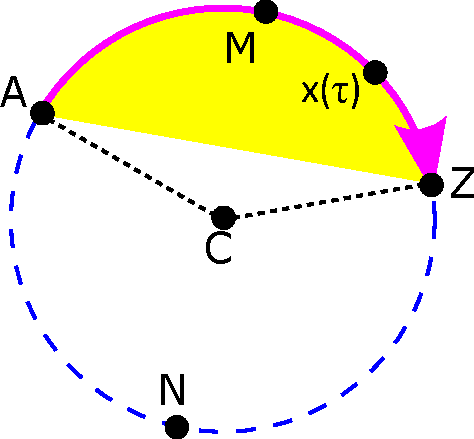
\includegraphics{arc.pdf}
  \caption{Основные элементы круговой дуги}
  \label{fig:app.arc}
\end{figure}

Знак параметра $\beta$
выберем положительным для дуг,
идущих против часовой стрелки
($\beta < 0$ на рис.~\ref{fig:app.arc}).
Для отрезка прямой
$\beta=0$,
для половины круга
$\beta = \pm 1$,
а для часто встречающегося на практике
случая дуги в четверть круга
$\beta = \pm(\sqrt{2}-1)\approx \pm 0.41421 \dots$

В этих обозначениях формула для положения
произвольной точки
$x(\tau)$ дуги,
параметризуемой положением
$\tau \in[-1,+1]$,
может быть просто подобрана из общих соображений
и приобретает вид:

\begin{equation}
  \label{eq:bulge.x}
  x(\tau) =
  \frac{A+Z}{2} + \frac{Z-A}{2}\frac{\tau - i \cdot \beta}{1 - i \cdot \beta \tau}
\end{equation}

Очевидно,
$x(-1) = A$,
$x(+1) = Z$.
Несложно также найти середину дуги
$M$
(<<зенит>>,
$\tau=0$)
$$
M = \frac{A+Z}{2} - \frac{Z-A}{2}i\beta
\equiv
\frac{1+i \beta}2 A + \frac{1-i \beta}2 Z
$$
и <<надир>> N
($\tau=\infty$):
$$
N = \frac{A+Z}{2} - \frac{Z-A}{2} \frac{1}{i\beta}
\equiv
\frac{1+i \beta}{2 i \beta} A - \frac{1 - i \beta}{2 i\beta} Z
$$

Заметим, что <<анти-дуга>>
${\smile} ANZ$
опирается на те же точки
$A$ и $Z$,
но с другим значением кривизны
$$
\beta^- = -\frac{1}{\beta}
$$

Далее уже легко найти центр:
$$
C =
\frac{(1+i\beta)^2}{4i\beta}A
-
\frac{(1-i\beta)^2}{4i\beta}Z
$$
и радиус
$$
R = \left| \beta + \frac{1}\beta \right|
\frac{\left|A-Z \right|}4
$$

\section*{Периметр и площадь}

Длина
(периметр)
дуги
${\smile}AMZ$:
\begin{equation}
  \label{eq:buldge.perimeter}
  P_{\smile} =
  \left(1+\beta^2 \right)
  \frac{\arctg \beta}{\beta}
  \left| A - Z \right|
\end{equation}

Для дуг, близких к отрезку
($\beta \to 0$):
$$
P_{\smile} =
 \left(1+\frac{2}{3}\beta^2 - \frac{2}{15}\beta^4 + \frac{2}{35}\beta^6 +O(\beta^8)\right)
 \left| A - Z \right|
$$

Площадь кругового сегмента
$AMZ$:
\begin{equation}
  \label{eq:buldge.area.segment}
  S_{\smile}=
  \frac{\left(1 - \beta^2\right) \beta - \left(1+\beta^2\right)^2\arctg \beta}{8\beta^2}
  |A-Z|^2
\end{equation}

В пределе,
когда дуга вырождается в отрезок,
$$
S_{\smile}=
  \left(
    -\frac{1}{3} \beta - \frac{1}{15}\beta^3 +\frac{1}{105}\beta^5 + O(\beta^7)
  \right)|A-Z|^2
$$

Площадь треугольника
$\triangle AOZ$
(где $O$ --- начало координат)
\begin{equation}
  \label{eq:buldge.area.tri}
  S_{\triangle} =
  \frac{\operatorname{im}A\cdot\overline Z}{2}
  \equiv
  \frac{\operatorname{re} Z \cdot \operatorname{im} A - \operatorname{im} Z \cdot \operatorname{re} A}2
\end{equation}

Знак в формулах для элемента площади
\eqref{eq:buldge.area.segment}--\eqref{eq:buldge.area.tri}
выбран в соответствии с соглашениями об ориентации контуров
в DBS-файле,
см.~Приложение~\ref{app:dbs}.

Комбинируя формулы
\eqref{eq:buldge.perimeter}--\eqref{eq:buldge.area.tri}
для контура,
состоящего из отрезков прямых и дуг окружностей,
получаем соответственно периметр контура
$$
P_{\circ} =  \sum P_{\smile}
$$
и площадь
\textit{замкнутого}
контура
$$
S_{\circ} = \sum S_{\smile} + S_{\triangle}
$$

\subsection*{Разбиение дуги}

Произвольная точка
$x(\tau)$
делит дугу
${\smile}AMZ$
на две,
вершины которых естественно вычислять по формуле
\eqref{eq:bulge.x},
а значения кривизны определяются по формуле
$$
\begin{cases}
  \beta_{-}(\tau)= \tg \frac{\arg (1+i\beta)(1+i\beta\tau)}2
  \\
  \beta_{+}(\tau)= \tg \frac{\arg (1+i\beta)(1-i\beta\tau)}2
  \end{cases}
  ,
$$
причём функция
$\tg(1/2\arg z)$
может вычисляться без использования
трансцендентных функций:
\begin{equation}
  \label{eq:bulge.tgq}
  \tg \frac{\arg z}2 =
  \begin{cases}
    \frac{|z|-\operatorname{re} z}{\operatorname{im} z}, & \operatorname{re} z < 0
    \\
    \frac{\operatorname{im} z}{|z|+\operatorname{re} z}, & \operatorname{re} z \geqslant 0
  \end{cases}
\end{equation}

Кривизны поддуг
$\beta_{\pm}(\tau)$
удовлетворяют формуле тангенса суммы:
$$
\beta = \frac{\beta_{-}(\tau)+\beta_{+}(\tau)}{1-\beta_{-}(\tau)\cdot\beta_{+}(\tau)}
$$

В частном случае разбиения дуги пополам
(в <<зените>>)
$\tau=0$:
$$
\beta_{1/2}=
  \frac{\beta}{1+\sqrt{1+\beta^2}}
$$

\section*{Построение дуги по трем точкам}

Иногда нужно найти дугу по ее концам и точке $x$,
через которую она проходит.
Кривизна такой дуги однозначно определяется
углом $\measuredangle AxZ$:
$$
\beta(x) =
  \tg \frac{\arg \overline{x - A} \cdot \left(Z- x \right)}{2}
  ,
$$
и функция
$\tg(1/2\arg z)$
по-прежнему может вычисляться по формуле~
\eqref{eq:bulge.tgq}.

Параметр же
$\tau$,
задающий положение точки $x$
на этой дуге,
однозначно зависит от отношения
$|A-x|:|Z-x|$:
$$
\tau(x) =
  \frac{|A-x|-|Z-x|}{|A-x|+|Z-x|}
$$

\section*{Скорость движения по дуге}

Скорость $v(\tau)$
движения точки $x(\tau)$
по дуге при изменении $\tau$
легко находится как производная:
$$
v(\tau) =
  \frac{\partial x}{\partial \tau} =
  \frac{Z-A}{2}\frac{1+\beta^2}{\left(1 - i \beta \tau \right)^2}
$$
Отсюда
$$
|v(\tau)| =
  \frac{\left|Z-A\right|}{2}\frac{1+\beta^2}{1 + \beta^2 \tau^2}
  ,
$$
и скорость движения точки $x(\tau)$
по дуге оказывается неравномерной,
наибольшей в середине
и минимальной по краям:
$$
\frac{|v(0)|}{|v(\pm1)|} = 1+\beta^2
,
$$
и
$$
\lim_{\beta \to \pm \infty}
  \frac{|v(0)|}{|v(\pm1)|} =
  \infty
  ,
$$
что делает построение больших дуг непосредственно по формуле~
\eqref{eq:bulge.x}
непрактичным.
Разумеется,
несложно найти другой параметр
$\widetilde{\tau}$,
такой, что
$v(\widetilde{\tau}) = const$,
но тогда в зависимость
$\tau(\widetilde{\tau})$
будет входить тригонометрическая функция.
Можно подобрать более простое преобразование,
дающее
\textit{почти}
равномерное движение:
$$
\tau(\hat \tau) =
  \frac{\hat \tau}{1 + \frac{\sqrt{9+8\beta^2}-3}{4} \left(1 -  \hat \tau^2\right)}
$$
и параметр
$\hat \tau \in[-1,+1]$.
